\chapter{STL: Standard Template Library}

\section{STL overview}

\textbf{STL} is a software library for the \texttt{C++} programming language that
provides four main components:
\begin{itemize}
    \item Algorithms
    \item Containers
    \item Functional (or functors)
    \item Iterators
\end{itemize}

STL provides a ready-made set of containers that can be used with any built-in and
user-defined types that supports some elementary operations (copying and assignment,
which are synthetized for us by the compiler if we don't define). Containers implement
a \textbf{like-a-value} semantic.\\

When we use an object to initialize a container, or insert an object into a container,
a copy of that object value is placed in the container, not the object itself. Just
as when we pass an object to a non-reference parameter (pass-by-value), there is no
relationship between the element in the container and the object that was used to
initialize it, so subsequent changes to the object will not affect the element in the
container, and vice versa.\\

STL algorithms are independent of containers, which significantly reduces the complexity
of the library. This is obtained also by the use of iterators, which are used to access
the elements of a container.\\

STL achieves its results through the use of templates. This approach provides compile-time
polymorphism that is often more efficient than traditional run-time polymorphism. Modern
\texttt{C++} compilers are tuned to minimize abstraction penalties arising from the heavy
use of the STL.\\

\section{STL containers classes}

Containers classes share a common interface, which each of the containers extends in its 
on way. This common inteface make the library easier to learn, and also make it easier to
change the container type used in a program, as we need limited changes to the code.\\

Each kind of container offers a different set of performance and functionality trade-offs.
There are two main categories of containers:

\begin{itemize}
    \item \textbf{Sequential containers:} Let the programmer control the order in which the
    elements are stored and accessed. That order does not depend on the values of the elements
    but on their position.

    \item \textbf{Associative containers:} Store their elements based on the value of a key.
    Elements are retrieved efficiently according to their key value.
\end{itemize}

\begin{figure}[H]
    \centering
    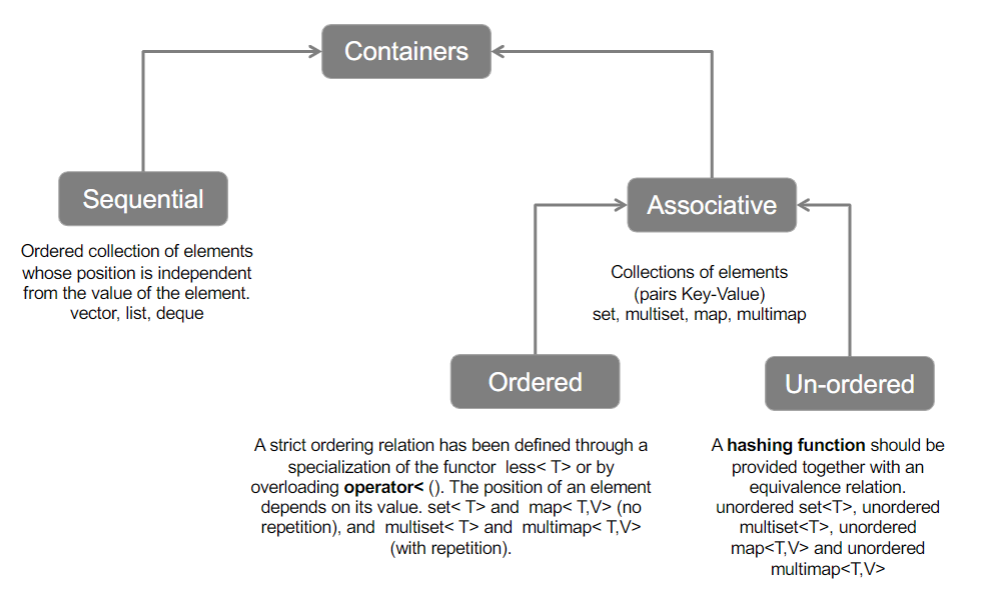
\includegraphics[width=0.9\textwidth]{figures/container_types.png}
    \caption{STL containers classes}
    \label{fig:containers}
\end{figure}

\subsection{Sequential containers}

The sequential containers provide fast sequential access to their elements. However, they offer 
different performance trade-offs relative to:
\begin{itemize}
    \item the costs to add or delete elements in the container
    \item the costs to perform non-sequential access to elements in the container
\end{itemize}

Some of the most important sequential containers are:

\begin{table}[H]
    \centering
    \begin{tabular}{|l|p{10cm}|}
    \hline
    \textbf{Container} & \textbf{Description} \\ \hline
    \texttt{vector} & Flexible-size array. Supports \textbf{fast random access}. Inserting or deleting elements other than the back is slow. \\ \hline
    \texttt{deque} & Double-ended queue. Supports \textbf{fast random access}. \textbf{Fast insert/delete at front or back}. \\ \hline
    \texttt{list} & Doubly linked list. Supports only \textbf{bidirectional sequential access}. \textbf{Fast insert/delete at any point}. \\ \hline
    \texttt{forward\_list} & Singly linked list. Supports only \textbf{sequential access in one direction}. \textbf{Fast insert/delete at any point}. \\ \hline
    \texttt{array} & Fixed-size array. Supports \textbf{fast random access}. Cannot add or remove elements. \\ \hline
    \texttt{string} & Specialized container (characters only), similar to \texttt{vector}. \textbf{Fast random access}. \textbf{Fast insert/delete at the back}. \\ \hline
    \end{tabular}
    \caption{Characteristics of different sequential containers in C++.}
    \label{table:containers}
\end{table}

\section{How are \texttt{vector}s implemented?}

As we know, a \texttt{vector} can hold an arbitrary number of elements of the same type, up to
the limit of available memory. The size of a vector can grow and shrink dynamically, as elements
are added or removed. The vector size changes by 3 mechanisms:

\begin{itemize}
    \item \textbf{Pushing elements:} When we add an element to the vector, the vector size grows.
    \item \textbf{Resizing:} This is done by the method \texttt{resize()}.
    \item \textbf{Assigning:} When we assign a vector to another vector, the size of the destination
    vector changes.
\end{itemize}

To support random access, the vector elements are stored in a contiguous block of memory. Given that
elements are contiguous, and that the size of the container is flexible, when we add an element if
there is no room for it:

\begin{itemize}
    \item the container must \textbf{allocate new memory} to hold the existing elements plus the
    new one.
    
    \item \textbf{copy} the elements from the old location into the new space.
    
    \item \textbf{add} the new element.
    
    \item \textbf{deallocate} the old memory.
\end{itemize}

To avoid these costs, library implementators use allocation strategies that reduce the number of
times the container is reallocated. One of them is, when new memory is needed, allocate capacity
beyond what is immediately needed. The container holds this storage in reserve and uses it to
allocate new elements as they are added. This allocation strategy is dramatically more efficient
that reallocating the container every time a new element is added.\\

\subsection{Adding elements to a vector}

There are 3 main operations that occur when we add an element to a vector:

\begin{itemize}
    \item \textbf{Reserve}
    \item \textbf{Resize}
    \item \textbf{Push back}
\end{itemize}

\subsubsection{\texttt{reserve(unsigned newalloc)}}

This method reserves memory for \texttt{newalloc} elements. If the requested size is less than
or equal to the current capacity, the method does nothing. Otherwise, it allocates memory for
\texttt{newalloc} elements, copies the existing elements into the new memory, and deallocates
the old memory.\\

The complexity of this method is linear in the number of elements in the vector.

\subsubsection{\texttt{resize(unsigned newsize)}}

Given \texttt{reserve}, \texttt{resize} is easy. While the first deals with the memory allocation,
\texttt{resize} deals with the element values. The \texttt{resize} goal is to resereve 
\texttt{newsize} elements, and fill the elements with indeces between sz and \texttt{newsize-1}
with the default value of the element type.\\

The complexity of this method is linear in the argument \texttt{newsize}.

\subsubsection{\texttt{push\_back(T val)}}

This method adds a new element with value \texttt{val} to the end of the vector. If there is 
enough room, it simply increments the size of the vector and copies the new element into the
pointer after the last previous element. If there is not enough room, it calls \texttt{reserve} 
with twice the current capacity, copies the elements into the new memory, and adds the new element.\\

The complexity of this method is linear in the number of elements in the vector.

\subsection{Vector complexity: final considerations}

Working with vectors implies that \texttt{push\_back} worst case complexity is linear in the 
number of elements in the vector. However, the amortized (average) complexity of 
\texttt{push\_back} is constant. This is because the cost of reallocation is spread over the
number of insertions.\\

Also, random access on vectors is constant time $O(1)$, as the elements are stored in a 
contiguous block of memory. Insert in the middle worst and average cases are $O(N)$.

\subsection{Range checking}

Ideally, we would like to have range checking on vectors. However, STL does not provide it
by default. Why is this? Because range checking is expensive, and the STL designers wanted
to keep the cost of using vectors low.\\

In general:

\begin{itemize}
    \item Range checking costs in speed and code size.
    \item Some projects need optimal performance: think huge (e.g., Google) and tiny (e.g.,
    embedded systems).
    \item The standard must serve everybody. You can build checked on top of optimal, but
    not the other way around.
\end{itemize}

\section{Sequential contaniers overview}

As we saw before, sequential containers provide efficient, flexible memory managememt. The strategies
that containers use for storing their elements have inheren, and sometimes significant, impact
on the efficiency of operations like adding or removing elements. In some cases, these strategies
also affect whether a particular container supplies a particular operation.

Based on amortized complexity, the following table provides a comparison of each sequential 
container:

\begin{figure}[H]
    \centering
    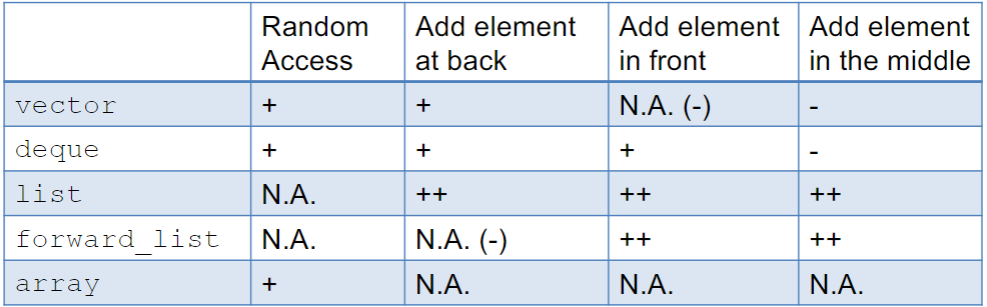
\includegraphics[width=0.8\textwidth]{figures/sequential_comparison.png}
    \caption{A comparison of the STL sequential containers}
    \label{fig:sequential-comparison}
\end{figure}

\textbf{Note:} the operation \textbf{add in the middle} assumes you have access (an iterator) to
the element before the one you will insert.\\

The \texttt{list} container implements a doubly-linked list, while the \texttt{forward\_list} 
implements a singly-linked list.Both are designed to make it fast to add or remove an element
anywhere in the container, but in exchange, these types do not support random access to
elements. Also, the memory overhead for these containers is significant.

\begin{figure}[H]
    \centering
    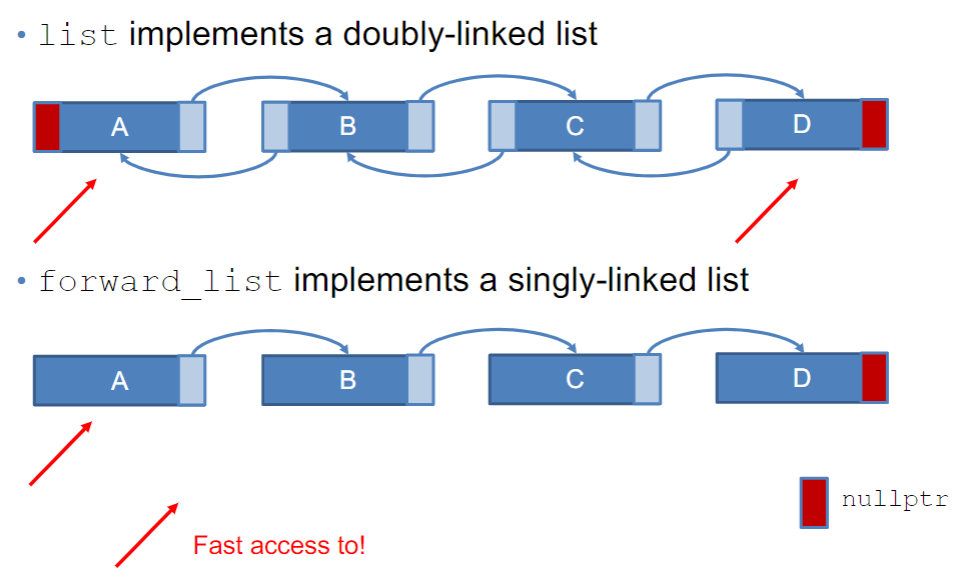
\includegraphics[width=0.8\textwidth]{figures/linked_lists.png}
    \caption{\texttt{list} and \texttt{forward\_list}}
    \label{fig:list_forward-list}
\end{figure}

A \texttt{deque} is a more complicated data structure. Like \texttt{string} and \texttt{vector},
it supports \textbf{fast random access}, and \textbf{adding} or \textbf{removing} elements in the
\textbf{middle} of a \texttt{deque} is an expensive operation. Adding or removing elements at
either the \textbf{front or end} is a fast operation, comparable to a list or \textbf{forward\_list}.\\

The \texttt{forward\_list} and \texttt{array} types were added by \texttt{C++ 11}. The first one
is comparable with a \texttt{list}, but it does not have the \texttt{size} operation and is more
memory efficient. In exchange, it can only be accessed from the \textbf{begin to end} (cannot move
backwards). On the other hand, an \texttt{array} is a safer, easier-to-use alternative to built-in
arrays and has a fixed size, but it does not support operations to add and remove elements or to
resize.

\subsection{Which one to use?}

It is best to use \texttt{vector} unless there is a good reason to prefer another container. If 
you need lots of small elements and space overhead matters, don't use \texttt{list} or
\texttt{forward\_list}. If the program requires random access to elements, use \texttt{vector}
or \texttt{deque}. If the program needs to insert or delete elements in the middle of the container,
use a \texttt{list} or a \texttt{forward\_list}. If the program needs to insert or delete elements
at the front and the back, but not in the middle, use \texttt{deque}.\\

There are some gray cases. If the program needs to insert elements in the middle of the container
only while reading input (e.g., to keep them in order), and subsequently needs random access to
the elements:
\begin{itemize}
    \item First decide whether you actually need to add elements in the middle of the container. It
    is often easier to append to a \texttt{vector} and then call the library \texttt{sort} function
    to reorder the container when you are done with the input.

    \item If you must insert into the middle, consider using a \texttt{list} for the input phase.
    Once the input is complete copy the \texttt{list} into a \texttt{vector}.
\end{itemize}

If the program needs random access and needs to insert and delete elements in the middle, evaluate 
the relative cost of accessing the elements in a \texttt{list} of \texttt{forward\_list} versus
the cost of inserting or deleting elements in a \texttt{vector} or \texttt{deque}.\\

In general, the predominant operation of the application (whether it does more access, more
insertion or more deletion) will determine the choice of the container type. Application 
performance testing is usually needed.\\

\textbf{ADVICE:} If ypu are not sure which container to use, write your code using only operations
common to \texttt{vector} and \texttt{list}:
\begin{itemize}
    \item Use iterators, not subscripts.
    \item Avoid random access to elements.
\end{itemize}

This way, the code could be changed easily!

\subsection{Container commont types}

The following table shows some common types between containers:

\begin{figure}[H]
    \centering
    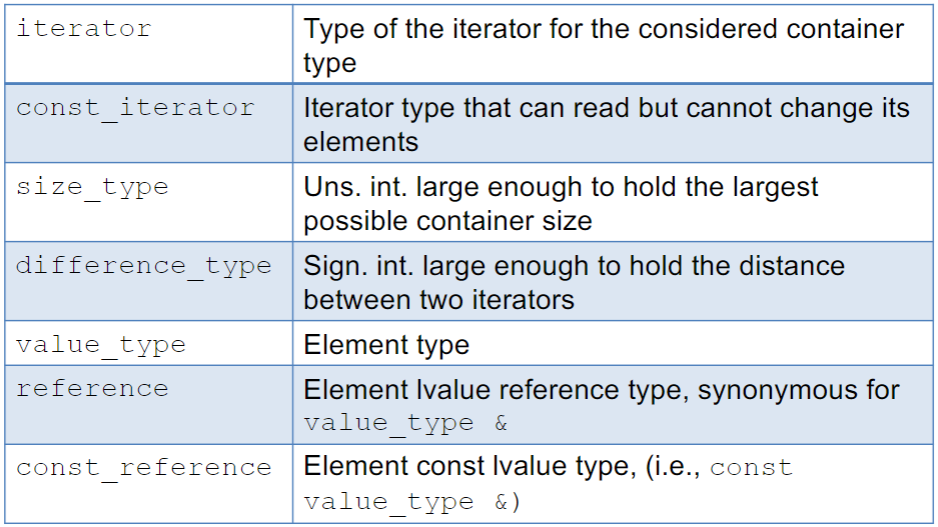
\includegraphics[width=0.8\textwidth]{figures/container_common_types.png}
    \caption{Container common types}
    \label{fig:common_types_container}
\end{figure}

\subsection{Container common operations}

The following table shows the containers common operations:

\begin{table}[H]
    \centering
    \begin{tabular}{@{}ll@{}}
    \toprule
    \textbf{Operation}              & \textbf{Description}  \\ \midrule                                                                           
    \texttt{C c;}                   & Default constructor, empty container                                                                       \\
    \texttt{C c1(c2);}              & Construct c1 as a copy of c2                                                                               \\
    \texttt{C c(b, e);}             & Copy elements from the range denoted by the iterators \\
                                    & b and e (no for \texttt{array})  \\
    \texttt{C c\{a, b, c, ...\};}   & List initialize c                                                                                         \\
    \texttt{c.size()}               & Number of elements in c (no for \texttt{forward\_list})                                                   \\
    \texttt{c.max\_size()}          & Maximum number of elements c can hold                                                                     \\
    \texttt{c.empty()}              & \texttt{true} if c has no elements, \texttt{false} otherwise                                              \\
    \texttt{c.insert(args)}         & Copy element(s) as specified by args in c                                                                 \\ 
    \texttt{c.emplace(inits)}       & Use inits to construct an element in c                                                                    \\
    \texttt{c.erase(args)}          & Remove element(s) specified by args                                                                       \\
    \texttt{c.clear()}              & Remove all elements from c                                                                                \\
    \texttt{==}, \texttt{!=}        & Equality                                                                                                  \\
    \texttt{<}, \texttt{>}, \texttt{<=}, \texttt{>=} & Relationals (no for unordered associative containers)                                    \\ 
    \texttt{c.begin()}, \texttt{c.end()}  & Return iterator to the first/one past element in c \\
    \texttt{c.cbegin()}, \texttt{c.cend()} & Return \texttt{const\_iterator} \\
    \texttt{reverse\_iterator} & Iterator that addresses elements in reverse order \\
    \texttt{const\_reverse\_iterator} & Reverse iterator read-only \\
    \texttt{c.rbegin()}, \texttt{c.rend()} & Iterator to the last, one past the first element in c \\
    \texttt{c.crbegin()}, \texttt{c.crend()} & Return \texttt{const\_reverse\_iterator} \\ \bottomrule
    \end{tabular}
    \caption{Container operations in STL}
\end{table}

Since \texttt{C++ 20}, the very same iterators can be obtained through the \texttt{<ranges>} library:

\begin{itemize}
    \item \texttt{ranges::begin(c)}, \texttt{ranges::end(c)}
    \item \texttt{ranges::cbegin(c)}, \texttt{ranges::cend(c)}
    \item \texttt{ranges::rbegin(c)}, \texttt{ranges::rend(c)}
    \item \texttt{ranges::crbegin(c)}, \texttt{ranges::crend(c)}
\end{itemize}

These are more helpful with functions that use both the begin and end iterators. For example,
consider the \texttt{sort} function:\\

\begin{lstlisting}[language=C++]
vector<double> v = {3, 7, 9.2, 44.3};
sort(v.begin(), v.end());
\end{lstlisting}

This now can be written as:\\

\begin{lstlisting}[language=C++]
#include <ranges>

vector<double> v = {3, 7, 9.2, 44.3};
ranges::sort(v);  // sort is a function of <algorithm>
\end{lstlisting}

\subsection{Creating a container}

Each container is defined in a header file with the same name as the type of container.
Note that containers are class templates, so you must specify the type of elements that
the container will hold. For example:\\

\begin{lstlisting}[language=C++]
#include <vector>
#include <list>
#include <deque>

vector<int> vi;  // vector of integers
list<string> ls; // list of strings
deque<double> vd; // deque of doubles
\end{lstlisting}

Almost any type can be used as element type of a sequential container. Some container operations
impose requirements of their own on the element type. In other words, we can define a container
for a type that does not support an operation-specific requirememt, but we can use an operation
only if the element type supports it.

\subsection{Iterators}

Iterators have also a common interface. All the iterators let access an element from a container
providing the dereference operator and allow to move from one element to the next through the
increment operator.\\

The following table shows the common operations of iterators:

\begin{figure}[H]
    \centering
    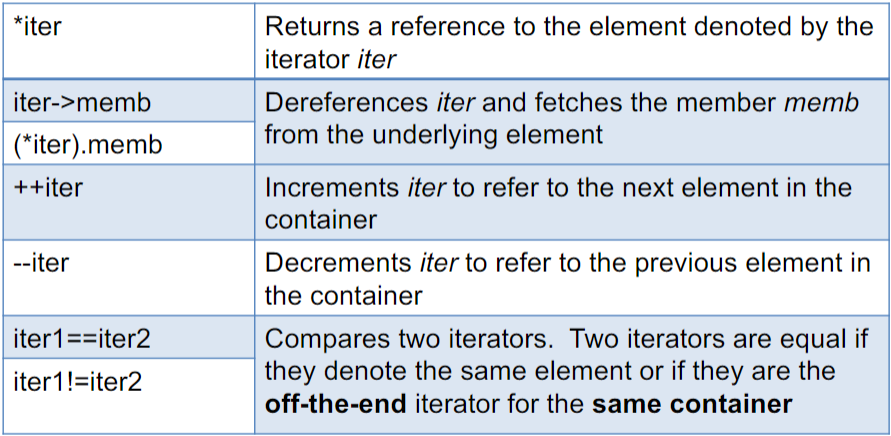
\includegraphics[width=0.8\textwidth]{figures/it_common_ops.png}
    \caption{Common operations of iterators}
    \label{fig:it_common_ops}
\end{figure}

Also for the containers that support random access, we have the following operations:

\begin{figure}[H]
    \centering
    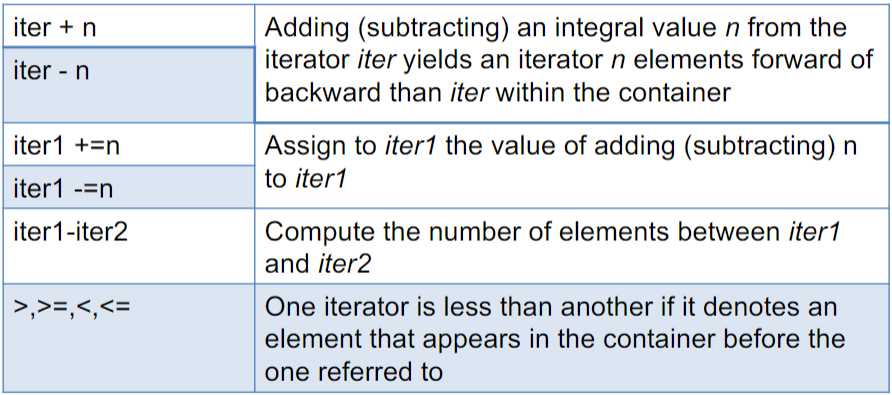
\includegraphics[width=0.8\textwidth]{figures/it_random_access.png}
    \caption{Random access operations}
    \label{fig:it_random_access}
\end{figure}

The previous table only apply to iterators for \texttt{string}, \texttt{vector}, \texttt{deque}
and \texttt{array}.

\subsubsection{Iterator ranges}

These are denoted by a pair of iterators, each of which referers to an element, or one past the
element, in the same container. They are often referred to as begin and end, or first and last.
In an iterator range we have a left-closed, right-open interval $[begin, end)$.\\

We have some nice properties of iterator ranges:

\begin{itemize}
    \item If begin equals end, the range is empty.
    \item If begin is not equal to end, there is at least one element in the range.
    and begin refers to the first element in that range.
    \item We can increment begin som number of times until it equals end.
\end{itemize}

For example:

\begin{lstlisting}[language=C++]
vector<int> v = {1, 2, 3, 4, 5};

for (auto p = v.begin(); p != v.end(); ++p)
    cout << *p << endl;

// or

p = v.begin();
while (p != v.end())
    cout << *p++ << endl;
\end{lstlisting}

\subsubsection{Reverse iterators}

Most containers provide reverse iterators, i.e., an iterator that goes backward through a 
container and inverts the meaning of the iterator operations. For example, incrementing a
reverse iterator moves it to the previous element, and decrementing it moves it to the next
element.

\subsection{Assignment operator}

The assignment operator replaces the entire range of elements in the left-hand container with
copies of the elements in the right-hand container. The left-hand container must be the same
type as the right-hand container, and the element type must be assignable. After an assignment,
the left-hand container is equal to the right-hand container.\\

The following table shows operations related to the assignment operator in containers:

\begin{figure}[H]
    \centering
    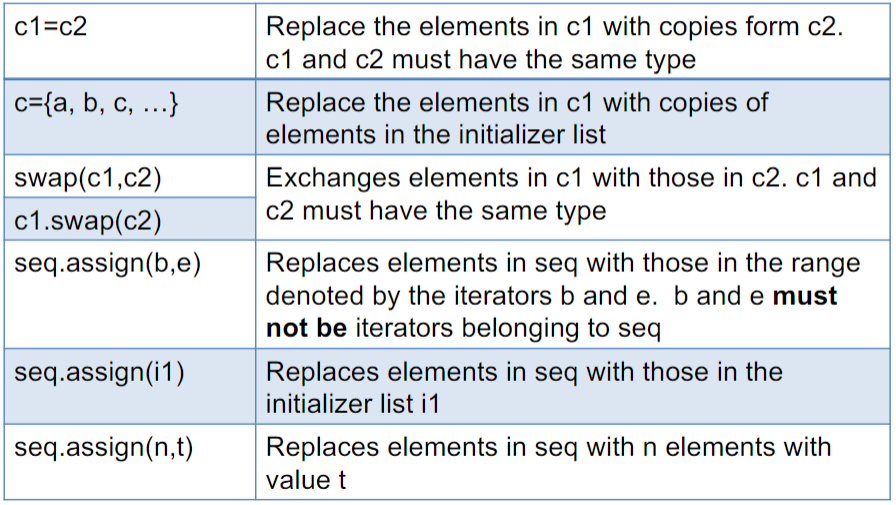
\includegraphics[width=0.8\textwidth]{figures/assignment_ops.png}
    \caption{Operations related to the assignment operator}
    \label{fig:assignment_ops}
\end{figure}

\subsubsection{Using \texttt{swap}}

The \texttt{swap} operation exchanges the elements in two containers. The containers must be of
the same type and have the same element type. After the operation, the elements in the two 
containers are exchanged, but the containers themselves are not changed.\\

For example:\\

\begin{lstlisting}[language=C++]
vector<int> v1 = {1, 2, 3, 4, 5};
vector<int> v2 = {6, 7, 8, 9, 10};

swap(v1, v2);  // v1 = {6, 7, 8, 9, 10}, v2 = {1, 2, 3, 4, 5}
\end{lstlisting}

With the exception of \texttt{array}, the \texttt{swap} operation is a constant-time operation.
Swapping two arrays does exchange the elements, and it requires time proportional to the number
of elements in the array, complexity $O(N)$.\\

The fact that elements are not moved means that iterators, reference and pointers into the 
containers are not invalidated by the \texttt{swap} operation. They will refer to the same
elements as they did before the operation, but after the swap, those elements will be in a
different container.\\

In \texttt{C++ 11}, the containers offer both a member function and a non-member function to
perform the swap operation. The member function is \texttt{c1.swap(c2)}, and the non-member
function is \texttt{swap(c1, c2)}. As a matter of habit, is better to use the non-member
function, as it is more flexible and can be used with any two containers of the same type.

\subsection{Container size operations}

Container types have three size-related operations:

\begin{itemize}
    \item \texttt{size()} returns the number of elements in the container.
    \item \texttt{empty()} returns a bool that is true if the size is zero, and false otherwise.
    \item \texttt{max\_size()} returns the maximum number of elements that the container can hold.
\end{itemize}

Note that \texttt{forward\_list} does not have a \texttt{size()} operation, but it does have
\texttt{max\_size()} and \texttt{empty()} operations.

\subsection{Relational operators}

Every container type supports the equality operators \texttt{==} and \texttt{!=}. With 
the exception of unordered associative containers, all container types also support the
inequality operators \texttt{<}, \texttt{>}, \texttt{<=}, and \texttt{>=}. The right-hand
and left-hand containers must be of the same type, and must hold elements of the same type.\\

Comparing two containers performs a pairwise comparison of the elements in the containers.
If both containers are the same size and all the elements in the containers are equal, the
containers are equal, otherwise, they are not. If the containers have different sizes, but
every element of the smaller one is equal to the corresponding element of the larger one,
then the smaller container is less than the larger one. If neither container is an initial
subsequence of the other, then the comparison is based on the first element that differs. 
This is called \textbf{lexicographical comparison}.\\

Note that instead of relying on \texttt{==} and \texttt{!=}, it is often better to use the
\texttt{equal} algorithm from the \texttt{<algorithm>} header. This algorithm is more flexible
and can be used with any two containers of the same type. In this case, you might also specify
a binary function to compare the elements.

\subsection{Adding elements to a sequential container}

Excepting \texttt{array}, all sequential containers provide flexible memory management. We can add
of remove elements dynamically changing the size of the container at run time.

\begin{table}[H]
\centering
\begin{tabular}{|l|p{11cm}|}
\hline
\textbf{Operation} & \textbf{Description} \\ \hline
\texttt{c.push\_back(t)} & Creates an element with value \texttt{t} or constructed from arguments at the end of \texttt{c}. \\ \hline
\texttt{c.emplace\_back(args)} & Creates an element with value \texttt{t} or constructed from arguments at the end of \texttt{c}. \\ \hline
\texttt{c.push\_front(t)} & Creates an element with value \texttt{t} or constructed from arguments at the front of \texttt{c}. \\ \hline
\texttt{c.emplace\_front(args)} & Creates an element with value \texttt{t} or constructed from arguments at the front of \texttt{c}. \\ \hline
\texttt{c.insert(p, t)} & Creates an element with value \texttt{t} or constructed from arguments \textbf{before} the element denoted by iterator \texttt{p}. \\ \hline
\texttt{c.emplace(p, args)} & Creates an element with value \texttt{t} or constructed from arguments \textbf{before} the element denoted by iterator \texttt{p}. \\ \hline
\texttt{c.insert(p, n, t)} & Creates \texttt{n} elements with value \texttt{t} \textbf{before} the element denoted by iterator \texttt{p}. \\ \hline
\texttt{c.insert(p, b, e)} & Inserts the elements from the range denoted by the iterators \texttt{b} and \texttt{e} \textbf{before} the element denoted by iterator \texttt{p}. \texttt{b} and \texttt{e} may not be in \texttt{c}. \\ \hline
\texttt{c.insert(p, \{i1\})} & \texttt{i1} is a braced list of element values. Inserts the elements \textbf{before} the element denoted by iterator \texttt{p}. \\ \hline
\end{tabular}
\caption{Adding Elements to a Sequential Container}
\label{tab:adding_elements}
\end{table}

When we use these operations, we must remember that the containers use different sttrategies for 
allocating elements and that these strategies affect performance:

\begin{itemize}
    \item Adding elements anywhere but at the end of a vector or string, or anywhere but the beginning
    or end of a deque, requires elements to be moved.
    \item Adding elements to a vector or string may cause the entire object to be reallocated.
    \item Reallocating an object requires allocating new memory and moving elements from the old space
    to the new space.
\end{itemize}

\subsubsection{How a \texttt{deque} works}

A \texttt{deque} is a double-ended queue. It supports fast random access, and fast 
insert and delete at the front or back. The \texttt{deque} organizes its elements in
chunks of memory referred by a sequence of pointers. It guarantees amortized constant
time for adding or removing elements at the front or back, but inserting or removing
elements in the middle is slow.\\

The worst case complexity for \texttt{push\_back} and \texttt{push\_front} is $O(N)$.

\begin{figure}[H]
    \centering
    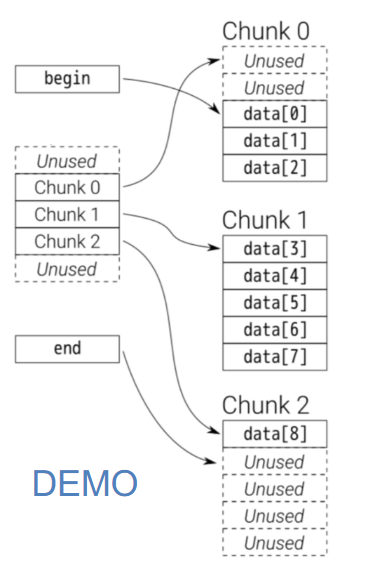
\includegraphics[width=0.4\textwidth]{figures/deque.png}
    \caption{How a \texttt{deque} works}
    \label{fig:deque}
\end{figure}

\subsubsection{Adding elements in the middle of a container}

Adding elements in the middle of a container is an expensive operation for all containers
except \texttt{list} and \texttt{forward\_list}. \\

To insert an element in the middle of a container, we rely on the \texttt{insert} operation.
It lets us insert one or more elements at any point in the container. The \texttt{insert}
is supported for \texttt{vector}, \texttt{string}, \texttt{deque}, and \texttt{list}, and
\texttt{forward\_list} provides specialized versions.\\

The operator \texttt{insert} takes an iterator as its first argument, which indicates where in
the container to put the element(s) (any position, including one past the end). Element(s) is/are
inserted before the position denoted by the iterator (the iterator might refer to a non-existant
element off the end of the container). It return an iterator to the first element inserted.\\

For example:

\begin{lstlisting}[language=C++]
vector<int> v = {1, 2, 3, 4, 5};

auto it = v.begin();
++it;  // it points to the second element

v.insert(it, 42);  // v = {1, 42, 2, 3, 4, 5}
\end{lstlisting}

We can use the return value of \texttt{insert} to insert multiple elements:

\begin{lstlisting}[language=C++]
list<string> lst;
auto iter = lst.begin();

while (cin >> word)
    iter = lst.insert(iter, word);
\end{lstlisting}

This is equivalent to using \texttt{push\_front}.

\subsection{Accessing elements}

We can access elements of a container using the following operations:

\begin{itemize}
    \item \texttt{c.back()}: returns a reference to the last element in \texttt{c}. It is undefined
    if \texttt{c} is empty.
    \item \texttt{c.front()}: returns a reference to the first element in \texttt{c}. It is undefined
    if \texttt{c} is empty.
    \item \texttt{c[n]} and \texttt{c.at(n)}: returns a reference to the element at 
    position \texttt{n} in \texttt{c}. It is undefined if \texttt{n} is out of range.
\end{itemize}

For example:

\begin{lstlisting}[language=C++]
vector<int> v = {1, 2, 3, 4, 5};

if (!v.empty()) {
    auto val1 = v.front();  // val1 = 1, equivalent to *v.begin()
    auto val2 = v.back();   // val2 = 5, equivalent to *(v.end() - 1)
    auto val3 = v[2];       // val3 = 3
    auto val4 = v.at(2);    // val4 = 3
}
\end{lstlisting}

Note that the operators \texttt{[]} and \texttt{at()} are only supported for containers
that provide random access to their elements. Also, the \texttt{c.back()} is not supported
for \texttt{forward\_list}.\\

\textbf{IMPORTANT:} The members that access elements in a container return \textbf{references}.
This means that we can change the value of the element using the returned reference, but only if
the container is not \texttt{const}. For example:

\begin{lstlisting}[language=C++]
vector<int> v = {1, 2, 3, 4, 5};

v[2] = 42;  // v = {1, 2, 42, 4, 5}

auto &val = v.front();
val = 42;   // v = {42, 2, 42, 4, 5}

auto val2 = v.front(); 
val2 = 42;  // This does not change the value of the first element in v,
            // but the value of val2, as it is a copy of the first element.
\end{lstlisting}

\subsection{Removing elements}

We can remove elements from a container using the following operations:

\begin{figure}[H]
    \centering
    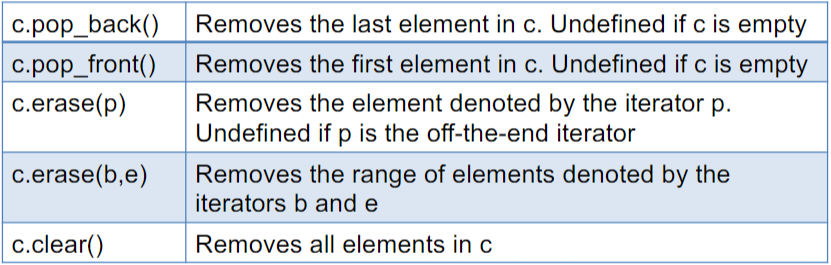
\includegraphics[width=0.8\textwidth]{figures/erasing_elems.png}
    \caption{Removing elements from a container}
    \label{fig:removing_elements}
\end{figure}

\subsubsection{\texttt{pop\_front} and \texttt{pop\_back}}

These functions remove the first and last elements of a container, respectively, and return
\texttt{void}. There is no \texttt{pop\_front} for \texttt{vector} and \texttt{string}, and
no \texttt{pop\_back} for \texttt{forward\_list}. We also cannot use \texttt{pop\_front} or
\texttt{pop\_back} on an empty container.

\subsubsection{\texttt{erase}}

This member function removes elements at a specified position in the container. We can delete
a single element or a range of elements. The function returns an iterator to the element that
follows the last element removed. For example:

\begin{lstlisting}[language=C++]
list<int> lst = {1, 2, 3, 4, 5};
auto it = lst.begin();

while (it != lst.end())
    if (*it % 2)
        it = lst.erase(it);
    else
        ++it;
\end{lstlisting}

\subsection{Iterator invalidation}

When we add or remove elements from a container, the iterators that refer to elements in the
container may be invalidated. An iterator is invalidated if the element to which it refers is
removed from the container. Using an invalidated iterator is a \textbf{serious error} that
can lead to undefined behavior.\\

After an operation that adds or removes elements from a container, iterators, pointers and 
references to a vector or string are invalid if the operation causes the container to reallocate.
If no reallocation happens indirect references to elements before the insertion remain valid;
those to elements after the insertion are invalid. It is \textbf{very risky} to rely on this!\\

\begin{itemize}
    \item Iterators, pointers and references to a \texttt{deque} are invalidated if we add
    elements anywhere but at the front or back of the container.
    \item If we add at the front of back, iterators are invalidated, but references and pointers
    to existing elements remain valid.
    \item Iterators, pointers and references to a \texttt{list} or \texttt{forward\_list} remain
    valid after an insertion. This includes the off-the-end and before-the-beginning iterators.
\end{itemize}

When we loop through a container and modify it, we must be careful to avoid using an invalidated
iterator. For example:\\

\begin{lstlisting}[language=C++]
vector<int> v = {1, 2, 3, 4, 5};
auto it = v.begin();

// This is ok, as we are refreshing the end iterator
while (it != v.end()) 
    if (*it % 2)
        it = v.erase(it);
    else
        ++it;

// This is not ok, as we are not refreshing the end iterator
auto end = v.end();
while (it != end)
    if (*it % 2)
        it = v.erase(it);
    else
        ++it;
\end{lstlisting}

\section{Adaptors}

Container adaptors ae interfaces created on top of a (limited) set of functionalities of a 
pre-existing sequential container, which provide a different API. When you declare the container
adaptors, you have an option of specifying which sequential container to use as underlying 
container.\\

We have three main container adaptors:

\begin{itemize}
    \item \texttt{stack}:
    \begin{itemize}
        \item This container provides a \textbf{last-in, first-out} (LIFO) access.
        \item You remove (pop) elements in the reverse order you insert (push) them.
        You cannot get any elements in the middle of the stack.
        \item Usually, this goes on top of a \texttt{deque}.
    \end{itemize}

    \item \texttt{queue}:
    \begin{itemize}
        \item Container providing a \textbf{first-in, first-out} (FIFO) access.
        \item You remove (pop) elements in the same order you insert (push) them.
        You cannot get any elements in the middle of the queue.
        \item Usually, this goes on top of a \texttt{deque}.
    \end{itemize}

    \item \texttt{priority\_queue}:
    \begin{itemize}
        \item Container providing \textbf{sorted-order} access to elements.
        \item You can insert (push) elements in any order, and then retrieve (pop) the 
        highest-priority element.
        \item Priority queues in \texttt{C++} STL use a heap structure internally, which in
        turn is basically \textbf{array-backed}; thus, usually goes on top of a \texttt{vector}.
    \end{itemize}
\end{itemize}

\section{Associative containers}

Associative containers support the general container operations, but they do not support
the sequential-container position-specific operations, such as \texttt{push\_front}. Because 
the elements are stored based on their \textbf{keys}, these operations would be meaningless for
the associative containers. Nevertheless, they have:

\begin{itemize}
    \item Type aliases
    \item \textbf{Bidirectional iterators}
    \item Specific operations
    \item Hash functions (for unordered associative containers)
\end{itemize}

The main associative containers are:

\begin{itemize}
    \item For the header \texttt{<map>}:
    \begin{itemize}
        \item \texttt{map}: a collection of key-value pairs, where the keys are unique.
        \item \texttt{multimap}: a collection of key-value pairs, where the keys may not be unique.
    \end{itemize}

    \item For the header \texttt{<set>}:
    \begin{itemize}
        \item \texttt{set}: a collection of unique keys.
        \item \texttt{multiset}: a collection of keys that may not be unique.
    \end{itemize}

    \item For the header \texttt{<unordered\_map>}:
    \begin{itemize}
        \item \texttt{unordered\_map}: a map organized by a hash function, where the keys are unique.
        \item \texttt{unordered\_multimap}: a map organized by a hash function, where the keys may not be unique.
    \end{itemize}

    \item For the header \texttt{<unordered\_set>}:
    \begin{itemize}
        \item \texttt{unordered\_set}: a set organized by a hash function, where the keys are unique.
        \item \texttt{unordered\_multiset}: a set organized by a hash function, where the keys may not be unique.
    \end{itemize}
\end{itemize}

\subsection{\texttt{map}}

A \texttt{map} is a collection of key-value pairs, where the keys are unique. It is often referred
to as an associative array. An associative array is like a "normal" array, but instead of using
integers as indices, you can use any type of key.\\

Values in a \texttt{map} are found by a key and not by their position. For example, given a map
of names to phone numbers, we'd use a person's name as a subscript to fetch their phone number:\\

\begin{lstlisting}[language=C++]
map<string, string> phone_book;

phone_book["John"] = "123-456-7890";

cout << phone_book["John"] << endl;  // prints 123-456-7890
\end{lstlisting}

\subsubsection{Implementation of a \texttt{map}}

A \texttt{map} is implemented by red-black trees, self-balancing binary search trees. The
\texttt{map} is always sorted by its key according to the comparison function. The complexity
of the operations is logarithmic ($O(\log(n))$) in the size of the container.

\begin{figure}[H]
    \centering
    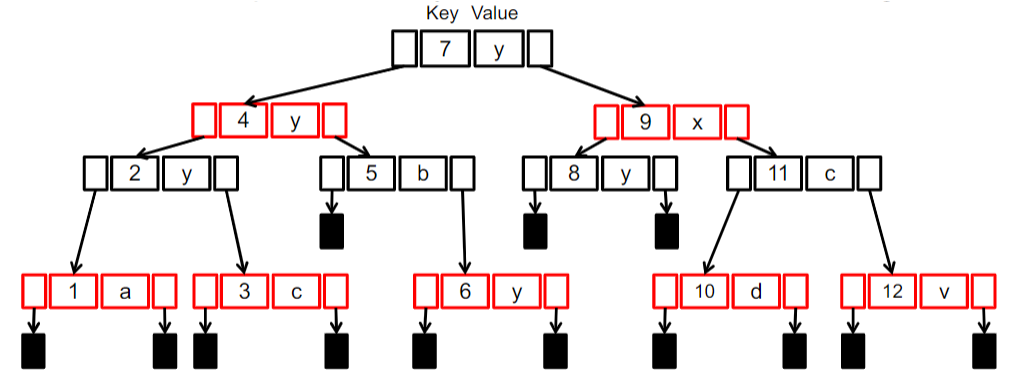
\includegraphics[width=0.8\textwidth]{figures/map.png}
    \caption{How a \texttt{map} works}
    \label{fig:map}
\end{figure}

\subsection{\texttt{set}}

A \texttt{set} is simply a collection of objects. A \texttt{set} is most useful when we simply
want to know whether an object is present in the collection or not.\\

For example, a business might have a set to hold the names of individuals sho have written
bad checks. When a new check is received, the business can quickly check the set to see if
the person has a history of writing bad checks:\\

\begin{lstlisting}[language=C++]
set<string> bad_check_writers;

if (bad_check_writers.find(name) != bad_check_writers.end())
    cout << "Do not accept check from " << name << endl;
\end{lstlisting}

\subsubsection{Implementation of a \texttt{set}}

A \texttt{set} is implemented by red-black trees, self-balancing binary search trees. The
\texttt{set} is always sorted by its key according to the comparison function. The complexity
of the operations is logarithmic ($O(\log(n))$) in the size of the container.

\begin{figure}[H]
    \centering
    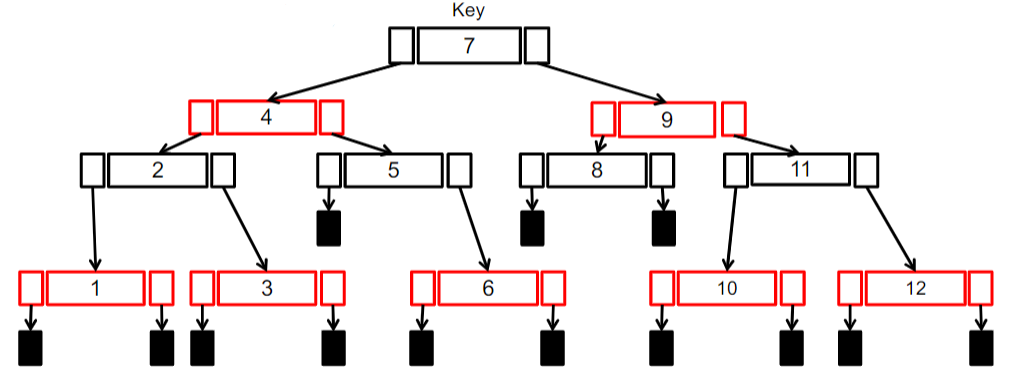
\includegraphics[width=0.8\textwidth]{figures/set.png}
    \caption{How a \texttt{set} works}
    \label{fig:set}
\end{figure}

\subsection{Associative vs sequential containers}

There are two main differences between associative and sequential containers:

\begin{itemize}
    \item The associative containers do not support the position-specific operations, such as
    \texttt{push\_front} and \texttt{push\_back}. Also they do not support constructors or insert
    operations that take an element value and a count.

    \item The asociative containers iterators are always bidirectional. Accessing \texttt{begin()}
    and \texttt{end()} is always $O(1)$, and incrementing or decrementing an iterator is always
    $O(1)$.
\end{itemize}

\subsection{Requirements on the key type}

For the \textbf{ordered containers}, the key type must define a way to compare the elements.
By default, the library uses the \texttt{<} operator to compare the keys, but we can also supply
our own \texttt{<} operation to use a strict weak ordering over the key type.\\

It has to be a strict weak ordering, which means that the relation must be:

\begin{itemize}
    \item \textbf{Irreflexive}: $a < a$ is always false.
    \item \textbf{Transitive}: If $a < b$ and $b < c$, then $a < c$.
    \item \textbf{Antisymmetric}: If $a < b$, then $b < a$ is false.
\end{itemize}

\subsection{The \texttt{pair} type}

The \texttt{pair} type is a simple way to combine two values into a single object. It is a
template class that takes two type parameters. It is defined in the \texttt{utility} header.
For example:\\

\begin{lstlisting}[language=C++]
pair<string, int> p1;  // default initialized

pair<string, int> p2("hello", 42);  // initialized to "hello" and 42

pair<string, int> p3 = make_pair("world", 42);  // initialized to "world" and 42
\end{lstlisting}

The \texttt{pair} type is used to return two values from a function. For example,
the \texttt{insert} operation on a \texttt{map} returns a \texttt{pair} of an iterator
to the element inserted and a bool that indicates whether the insertion was successful.\\

The data members of a \texttt{pair} are public, and can be accessed using the \texttt{first}
and \texttt{second} members. Note that the elements in a \texttt{map} are \texttt{pair}s.
We have a limited set of operations for \texttt{pair}:

\begin{figure}[H]
    \centering
    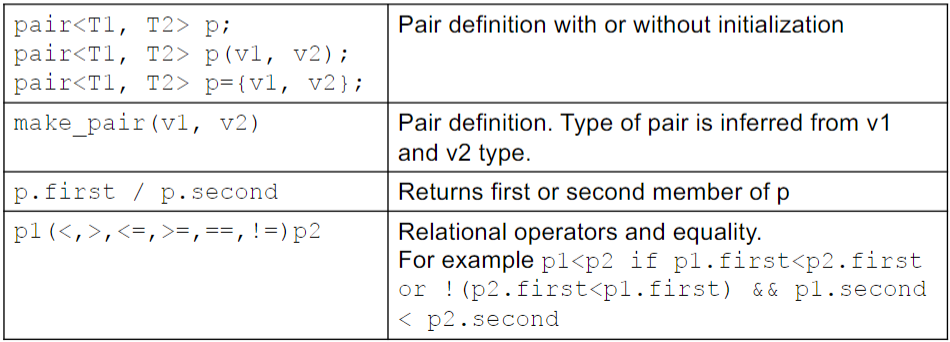
\includegraphics[width=0.8\textwidth]{figures/pair_ops.png}
    \caption{Operations for \texttt{pair}}
    \label{fig:pair_ops}
\end{figure}

\subsection{Associative container type aliases}

We have the following type aliases for the associative containers:

\begin{itemize}
    \item \texttt{key\_type}: the type of the key.
    \item \texttt{mapped\_type}: the type of the value.
    \item \texttt{value\_type}: it is the same as \texttt{key\_type} for \texttt{set} and
    a \texttt{pair} of \texttt{key\_type} and \texttt{mapped\_type} for \texttt{map}.
\end{itemize}

Note that the key is \texttt{const}, meaning that we cannot change the key of an element in
an associative container. For example, when we retrieve an element from a \texttt{map}, we can 
change the value of the element, but not the key. Look at the following example:\\

\begin{lstlisting}[language=C++]
map<string, int> m;

m["hello"] = 42;

auto it = m.find("hello");
if (it != m.end())
    it->second = 43;  // ok
it->first = "world";  // error
\end{lstlisting}

\subsection{Iterating over an associative container}

When we use an iterator to travers a map, multimap, set or multiset, the iterators yield 
elements in \textbf{ascending order} according to the key. For example, consider the following
code:\\

\begin{lstlisting}[language=C++]
map<string, int> m = {{"hello", 42}, {"world", 43}};
for (auto it = m.begin(); it != m.end(); ++it)
    cout << it->first << " " << it->second << endl;

// prints:
// hello 42
// world 43
\end{lstlisting}

\subsection{Adding elements to an associative container}

Because (unordered) \texttt{map} and (unordered) \texttt{set} contain unique keys, inserting
elements that are already present, has no effect:

\begin{figure}[H]
    \centering
    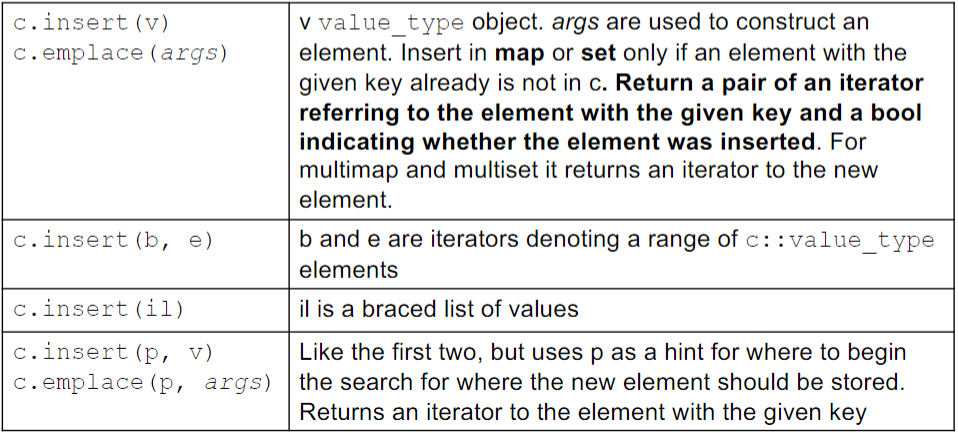
\includegraphics[width=0.8\textwidth]{figures/associative_add_ops.png}
    \caption{Operations for adding elements on associative containers}
    \label{fig:associative_add_ops}
\end{figure}

For example:

\begin{lstlisting}[language=C++]
vector<int> ivec = {2, 4, 6, 8, 2, 4, 6, 8};

set<int> set2;
set2.insert(ivec.cbegin(), ivec.cend()) // set2 has 4 elements
\end{lstlisting}

\subsection{Erasing elements}

We can erase one element or a range of elements by passing erase or an iterator pair:

\begin{figure}[H]
    \centering
    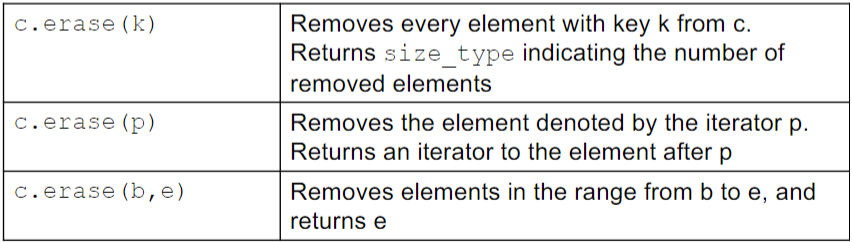
\includegraphics[width=0.8\textwidth]{figures/erasing_associative.png}
    \caption{Erasing ops on associative containers}
    \label{fig:erasing_associative}
\end{figure}

\subsection{Subscritping a \texttt{map}}

The \texttt{map} and \texttt{unordered\_map} containers provide the susbcript operator and a 
corresponding \texttt{at} function. The \texttt{set} types do not support subscripting because
there is no value associated with a key. We also cannot subscript a \texttt{multimap} or an
\texttt{unordered\_multimap} because there may be more than one value associated with a given key:

\begin{figure}[H]
    \centering
    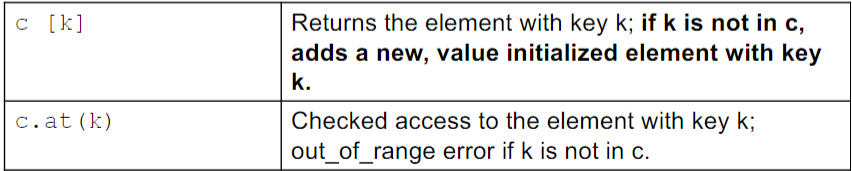
\includegraphics[width=0.8\textwidth]{figures/subscripting_map.png}
    \caption{Subscripting a map}
    \label{fig:map_subscript}
\end{figure}

\subsection{Accessing elements} 

We can use these operations to access elements on an associative container:

\begin{figure}[H]
    \centering
    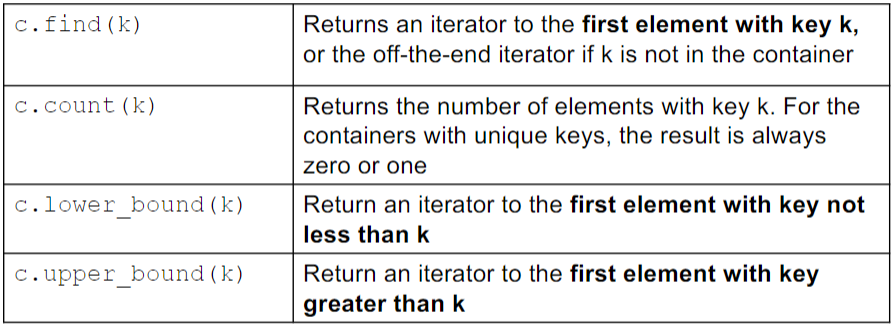
\includegraphics[width=0.8\textwidth]{figures/accessing_associative.png}
    \caption{Accessing elements on associative containers}
    \label{fig:accessig_associative}
\end{figure}

Note that lower and upper bound are not valid for unordered containers, in that case you can 
rely on \texttt{equal\_range}.

\subsection{\texttt{unordered\_map} \& \texttt{unordered\_set}}

The unordered associative containers are just a collection of buckets, each containing a variable
number of items. These containers use a \textbf{hash function} to map elements to buckets. Given
the item key, this identifies the proper bucket to store such item. All of the elements with a 
given hash value are stored in the same bucket, and all the elements with the same key (in the
multi-version) will be in the same bucket.

\begin{figure}[H]
    \centering
    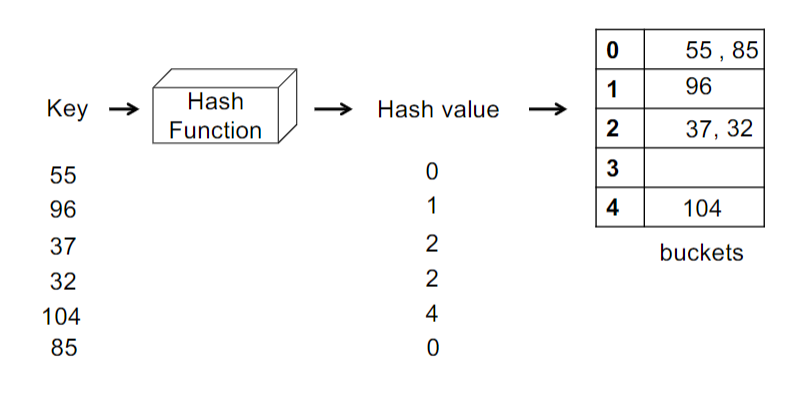
\includegraphics[width=0.6\textwidth]{figures/hash_working.png}
    \caption{How a hash works}
    \label{fig:hash_working}
\end{figure}

\begin{figure}[H]
    \centering
    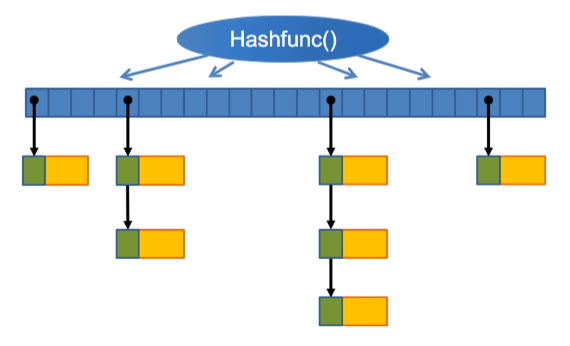
\includegraphics[width=0.6\textwidth]{figures/hash_diagram.png}
    \caption{Diagram of a map using a hash function}
    \label{fig:hash_diagram}
\end{figure}


The performance of an unordered container depends on the quality of its hash
function and on the number and size of its buckets. The average complexity is
constant ($O(1)$) and the worst case has a linear complexity $(O(N))$.\\

Rather than using comparison operation to organize their elements, these containers
use a hash function ans the key type's \texttt{==} operator. We should use an
unordered container if the key type is inherently unordered or if performance testing
reveals problems that hashing might solve.

\subsection{Complexities of operations}

You can choose the most suitable container in terms of complexity, depending on what
operations you need to apply on them:

\begin{figure}[H]
    \centering
    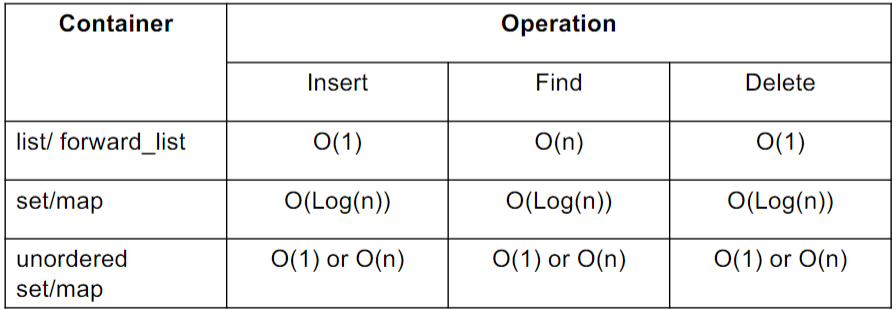
\includegraphics[width=0.8\textwidth]{figures/complexities_containers.png}
    \caption{Complexities of main operations}
    \label{fig:complexities_containers}
\end{figure}

\subsection{\texttt{map} vs \texttt{unordered\_map}}

If the most frequent operations of your application are \textbf{find, insert or delete} of 
single elements and you access through a key:

\begin{itemize}
    \item Use a \texttt{map} if you want to optimize the worst case complexity ($O(\log N)$ vs 
    $O(N)$)
    \item Use an \texttt{unordered\_map} if you want to optimize the average case complexity 
    ($O(1)$ vs $O(\log N)$)
\end{itemize}

